\chapter{\protect\hyperlink{:}{传播子与微扰}}
\addtocontents{toc}{\protect\hypertarget{:}{}}


在我们执行量子力学的时候，我们有一种方法是通过计算波函数以及作用在其上的算符。另外一种方法是直接考虑某一个给定过程的振幅，例如“对于一个起始于 $(t_y,y)$ 并且终止于 $(x,t_x)$ 的一个粒子的振幅”，我们将其记作 $\bra{x(t_x)}\ket{y(t_y)}$，这个振幅就是我们所说的传播子(propagator)。并且一个单粒子的传播子的数学表达我们可以使用粒子的运动方程的格林函数来表示。

\section{\protect\hyperlink{:}{格林函数}}
\addtocontents{toc}{\protect\hypertarget{:}{}}

这里我们将要先介绍一下格林函数的概念

首先对于一个微分方程，我们可以使用线性微分算子 $\hat{L}$ 来表示
\begin{equation*}
    \hat{L} x(t) = f(t)
\end{equation*}

我们将一个线性微分算子 $\hat{L}$ 的格林函数 $G(t,u)$ 通过一个方程定义为
\begin{equation*}
    \hat{L} G(x,t) = \delta (t - u)
\end{equation*}

给一个例子来描述一下
\begin{example}
    对于一个质量为 $m$ 弹性系数为 $K$ 的谐振子在一个随时间变化的影响 $f(t)$ 的作用下，其运动方程为 
    \begin{equation*}
        m\frac{d^2}{dt^2}{x} + Kx = f(t)
    \end{equation*}

    这里的线性微分算子为 $\displaystyle \hat{L} = m\frac{d^2}{dt^2} + K$，同时，我们可以通过叠加很多的 $\delta$ 函数来表示 $f(t)$，即
    \begin{equation*}
        f(t) = \int_0^\infty du f(u) \delta (t - u) 
    \end{equation*}
    
    这时，我将给出这个谐振子的格林函数
    \begin{equation*}
        \left[m\frac{d^2}{dt^2} + K\right]G(u,t) = \delta(t - u)
    \end{equation*}

    而原来的运动方程的解为
    \begin{equation*}
        x(t) = \int_0^\infty du G(u,t) f(u)
    \end{equation*}
\end{example}

在这里我们已经很明晰地看到，我们的格林函数需要两个变量，其中一个是我们所关心的量，在这里的例子里就是时间 $t$ ，而另外一个变量则是为了来描述我们的 $\delta(t - u)$ 函数的位置


\section{\protect\hyperlink{:}{量子力学中的传播子}}
\addtocontents{toc}{\protect\hypertarget{:}{}}

我们知道描述波函数 $\phi(x,t)$ 变化的方程是薛定谔方程 
\begin{equation*}
    \hat{H}\phi(x,t) = i\frac{\partial}{\partial t}\phi(x,t)
\end{equation*}

这里我们只考虑 $(1 + 1)$ 维的时空，接下来我们给出这个薛定谔方程的格林函数的形式
\begin{equation*}
    \phi(x,t_x) = \int dy G^{+}(x,t_x;y,t_y)\phi(y,t_y)
\end{equation*}

这里的 $G^{+}$ 被称为推迟格林函数(time-retarded Green's function)，所想表达的是
\begin{equation*}
    G^+ = 
    \begin{cases}
        G &\quad t_x > t_y \\
        0 &\quad t_x < t_y
    \end{cases} 
    = \theta(t_x - t_y)G
\end{equation*}

这样的定义将会避免粒子回到之前的时间里，很显然这是不符合物理的。

同理，我们也可以定义出超前格林函数(time-advanced Green's function)，
\begin{equation*}
    G^- =
    \begin{cases}
        G &\quad t_x < t_y \\
        0 &\quad t_x > t_y
    \end{cases}
    = \theta(t_y - t_x)G
\end{equation*}

在这里，我们的格林函数传播子将波函数从时空点 $(t_y,y)$ 演化到了时空点 $(t_x,x)$ ，这也是我们将其命名为传播子的原因。

此外，我们可以认为 $\phi(y,t_y),\phi(x,t_x)$ 是在 $(y,t_y),(x,t_x)$ 找到这个粒子的几率波幅，这样的话我们的传播子 $G^+(t_x,x;t_y,y)$ 将会是粒子在 $t_y$ 处于态 $\ket{y}$ ,并且在时刻 $t_x$ 处于态 $\ket{x}$ 的几率波幅，根据这个想法，我们可以将格林函数写为
\begin{equation*}
    G^+(t_x,x;t_y,y) = \theta(t_x - t_y) \bra{x(t_x)}\ket{y(t_y)}
\end{equation*}

而我们的老朋友波函数则是被表示为 $\phi(x,t_x) = \braket{x}{\phi(x)}$ ，这将会是粒子在 $(t_x,x)$ 被找到的概率波幅，因此当我们开始关注粒子将会从哪里开始时，我们的传播子将包含了更多的信息。

根据我们对于传播子 $G^{+}(t_x,x;t_y,y)$ 的定义，我们结合时间演化算符来计算一下
\begin{align*}
    G^{+}(t_x,x;t_y,y) &= \theta(t_x - t_y) \braket{x(t_x)}{y(t_y)} \\
    &= \theta(t_x - t_y)\bra{x}e^{-i\hat{H}(t_x - t_y)}\ket{y} \\
    &= \theta(t_x - t_y)\sum_n\bra{x}e^{-i\hat{H}(t_x - t_y)}\ket{n}\bra{n}\ket{y} \\
    &= \theta(t_x - t_y)\sum_n \phi_n(x)\phi_n^\star(y)e^{-iE_n(t_x - t_y)}
\end{align*}

接下来我们在计算完传播子的一般情况之后，再来计算一下在非相对论条件下，自由粒子的传播子。

我们知道，对于非相对论情况下的自由粒子，其哈密顿量,本征波函数方程和本征值为
\begin{align*}
    \hat{H} &= \frac{\hat{p}^2}{2m} \\
    \phi(x) &= \frac{1}{\sqrt{L}}e^{ipx} \\
    E_p &= \frac{p^2}{2m}
\end{align*}

在这样的情况下，传播子自然可以被写为
\begin{align*}
    G^{+}(t_x,x;t_y,y) &= \theta(t_x - t_y) L\int \frac{dp}{2\pi} \phi_p(x) \phi_p^\star(y) e^{-i\frac{p^2}{2m}(t_x - t_y)} \\
    &= \theta(t_x - t_y) L\int \frac{dp}{2\pi} e^{ip(x - y)} e^{-i\frac{p^2}{2m}(t_x - t_y)} \\
    &= \theta(t_x - t_y) L\int \frac{dp}{2\pi} e^{i[(x - y)p - \frac{(t_x - t_y)}{2m}p^2]} \\
    &= \theta(t_x - t_y) \sqrt{\frac{m}{2\pi i(t_x - t_y)}} e^{\frac{im(x - y)^2}{2(t_x - t_y)}}
\end{align*}


\section{\protect\hyperlink{:}{传播子的量子力学与微扰理论}}
\addtocontents{toc}{\protect\hypertarget{:}{}}

在前面的内容当中我们已经利用了我们对量子力学的了解来推导出单粒子传播子的一些特性。事实上，我们想扭转这种情况。如果我们从传播子开始，我们可以了解粒子的哪些信息？通过考虑格林函数的另一种形式，同样是空间的函数，但这次是在频率/能量域中。

接下来，我们将传播子从空间时空里转换到空间能量中，也就是 $G^{+}(x,y,E)$

我们假定粒子产生的时刻为 $t_y = 0$并且湮灭在时刻 $t_x = t$,因此我们的传播子形式为
\begin{equation*}
    G^{+}(t,x;0,y) = \theta(t) \sum_n \phi_n(x)\phi_n^\star(y)e^{-iE_n t}
\end{equation*}


接下来对时间和能量做一个傅里叶变换，有
\begin{align*}
    G^{+}(x,y,E) &= \int_{-\infty}^{\infty} \theta(t) \sum_n \phi_n(x)\phi_n^\star(y)e^{-iE_n t} e^{iEt} dt \\
    &= \int_{0}^{\infty}\sum_n \phi_n(x)\phi_n^\star(y)e^{i(E - E_n)t}
\end{align*}

为了方便，我们给我们的能量 $E_n$ 一个很小的虚部修正 $e^{-\epsilon t}$（$\epsilon > 0$）

于是，我们的传播子可以写为
\begin{align*}
    G^{+}(x,y,E) &= \sum_n \int_{0}^{\infty}\phi_n(x)\phi_n^\star(y)e^{i(E - E_n +i\epsilon)}dt \\
    &= \sum_n \frac{i\phi_n(x)\phi_n^\star(y)}{E - E_n +i\epsilon}
\end{align*}

当然，我们也可以计算出其连续形式，这主要取决于 $\theta(t)$
\begin{equation*}
    \theta(t) = i \int_{-\infty}^{\infty} \frac{dz}{2\pi}\frac{e^{-izt}}{z + i\epsilon}
\end{equation*}

借助这个，我们可以继续计算出其传播子的连续形式
\begin{align*}
    G^{+}(x,y,E) &= \int_{-\infty}^{\infty} \int_{0}^{\infty} \frac{i}{2\pi}e^{i(E - E_p -z)t} dt dz\\
    &= \int_{-\infty}^{\infty} \frac{i}{z + i \epsilon} \delta(E - E_p -z) dz \\
    &= \frac{i}{E - E_p + i\epsilon}
\end{align*}

在计算完之后，我们仔细看一看这些传播子能告诉我们一些什么样的信息，这里给出两个信息：
\begin{enumerate}
    \item 当 $E = E_n$，即能量等于某个本征态的能量的时候，将会出现奇点
    \item 奇点处的留数即为我们的 $i$ 倍波函数
\end{enumerate}

因此，我们可以断言，在我们写下了传播子之后，我们将会知道系统的能量以及波函数的信息。

事实上，我们的传播子在微扰计算当中能起到非常大的作用，在现实当中，很多的量子力学问题都是不能够精确求解的，所以我们发展出了微扰计算方法，这个方法当中，我们将系统的哈密顿量分为两部分：$\hat{H} = \hat{H}_0 + V$，这当中，一部分是被解出来的哈密顿量，另一部分则是微扰项。

回顾一下我们对于格林函数的定义并结合量子力学的薛定谔方程，我们可以将其写为
\begin{equation*}
    \left(\hat{H} - E\right) G = -i\delta(x - y)
\end{equation*}

将其写成矩阵形式,我们有 
\begin{equation*}
    \left(E - H\right)G = -I
\end{equation*}

因此，我们可以直接将格林函数写成
\begin{equation*}
    G = \frac{1}{E - H}
\end{equation*}

我们需要牢牢记住的一点是：格林函数描述的是一个粒子从 $y$ 传播到 $x$ 的过程。因此，格林函数使我们能够从传播粒子的角度来解释扰动问题，我们将问题的可解部分视为从一点传播到另一点的粒子，将扰动 $V$ 视为中断传播的散射过程。

基于这一点，我们将一个体系的哈密顿量进行分解
\begin{align*}
    G &= \frac{1}{E - H_0 - V} \\
    &= \frac{1}{E - H_0} + \frac{1}{E - H_0}V\frac{1}{E - H_0} + \frac{1}{E - H_0}V\frac{1}{E - H_0}V\frac{1}{E - H_0} + \cdots
\end{align*}

在这里面，我们已经解出亦或是可以解出的部分即为
\begin{equation*}
    G_0 = \frac{1}{E - H_0}
\end{equation*}

因此，我们可以将系统本身的格林函数写作
\begin{align*}
    G &= G_0 + G_0VG_0 + G_0VG_0VG_0 + \cdots\\
    &= G_0\left(1 + V G_0 + V G_0 V G_0 + \cdots\right) \\
    &= G_0\left(1 + \sum_{n = 1}^{\infty} (V G_0)^n\right) \\
    &= \frac{G_0}{1 - V G_0} \\
    &= \frac{1}{G_0^{-1} - V}
\end{align*}

注意到，这个最终结果是一个非微扰的结果，因为我们考虑到了其无穷项。

根据我们之前所描述的，我们已经将问题分解为了两个部分：可解部分视为从一点传播到另一点的粒子，将扰动 $V$ 视为中断传播的散射过程。

接下来我将给出三个图形来描述这个过程
\begin{figure}[hbpt]
    \begin{minipage}{0.3\textwidth}
        \centering
        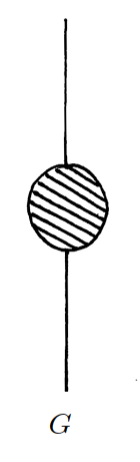
\includegraphics[width = 0.3\textwidth]{figure/总的格林函数.png}
    \end{minipage}
    \hfill
    \begin{minipage}{0.3\textwidth}
        \centering
        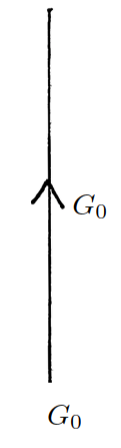
\includegraphics[width = 0.3\textwidth]{figure/自由粒子格林函数.png}
    \end{minipage}
    \hfill
    \begin{minipage}{0.3\textwidth}
        \centering
        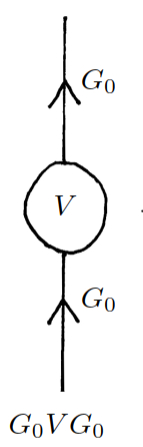
\includegraphics[width = 0.3\textwidth]{figure/一阶微扰格林函数.png}
    \end{minipage}
\end{figure}

基于此，我们可以给出格林函数的微扰展开形式
\begin{figure}[hbpt]
    \centering
    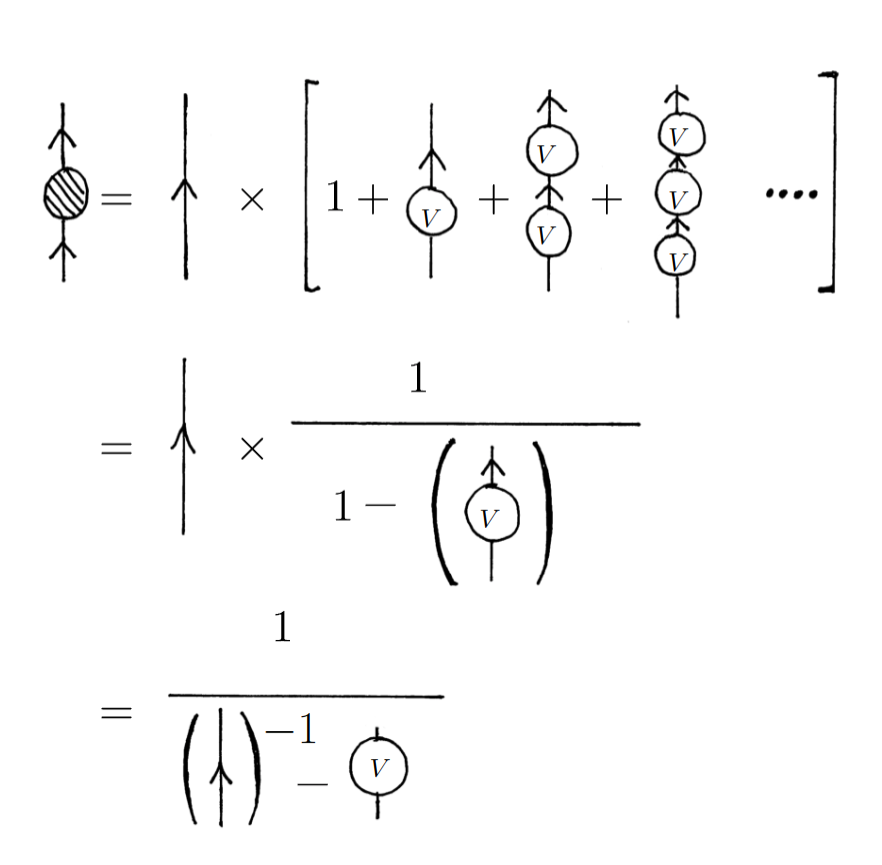
\includegraphics[width = 0.5\textwidth]{figure/格林函数微扰展开.png}
\end{figure}

这个微扰展开具有非常清晰的物理图像：
\begin{itemize}
    \item 第一项 $G_0$ 表示自由粒子从 $y$ 传播到 $x$，没有任何相互作用
    \item 第二项 $G_0VG_0$ 表示粒子从 $y$ 传播到某点，与势场 $V$ 发生一次相互作用，然后继续传播到 $x$
    \item 第三项 $G_0VG_0VG_0$ 表示粒子经历两次散射过程
    \item 以此类推，高阶项表示粒子经历多次散射
\end{itemize}

在实际计算中，我们通常截断这个级数到有限阶。例如，在一阶微扰近似下，我们有
\begin{equation*}
    G \approx G_0 + G_0VG_0
\end{equation*}

这对应于粒子最多经历一次散射的过程。微扰展开的有效性要求微扰项 $V$ 相对于 $H_0$ 足够小，使得高阶项可以忽略。

微扰论的一个重要应用是计算散射振幅。在量子场论中，我们将相互作用项视为对自由理论的微扰，通过计算费曼图来得到散射截面。每一个费曼图对应微扰展开中的一个特定项，而费曼传播子正是这些图的基本构建块。


事实上，我们在计算一个粒子的传播子时，我们并不容易知道粒子的位置信息，因此，我们将使用动量来表示
\begin{align*}
    G^{+}_0(p,t_x;q,t_y) &= \theta(t_x - t_y) \bra{p}\hat{U}(t_x - t_y)\ket{q} \\
    &= \theta(t_x - t_y) \bra{p}\hat{U}\ket{q}e^{-iE_{\vec{q}}(t_x - t_y)} \\
    &= \theta(t_x - t_y) \delta(p - q)e^{-iE_{\vec{q}}(t_x - t_y)}
\end{align*}

通过这个计算我们可以看出，自由粒子是不可以改变他的动量本征态的，受限制于 $\delta(p - q)$ 其形式只能是
\begin{equation*}
    G^{+}_0(p,t_x,t_y) = \theta(t_x - t_y)e^{-iE_{\vec{q}}(t_x - t_y)}
\end{equation*}

当然，这还是不够方便，如果我们使用的是动量和能量，这将会满足我们的实验数据
\begin{align*}
    G_0^{+}(p,E) &= \int dt e^{iEt}G_0^{+}(p,t,0) \\
    &= \int dt e^{iEt}\theta(t)e^{-i(E_{\vec{p}} + i\epsilon) t} \\
    &= \int_{0}^{\infty} \frac{i}{2\pi(z + i\epsilon)} e^{i(E - E_p -z)t}dt dz\\
    &= \int_{0}^{\infty} \frac{i}{(z + i\epsilon)} \delta(E - E_p -z) dz\\
    &= \frac{i}{E - E_p + i\epsilon}
\end{align*}

\section{\protect\hyperlink{:}{场的传播子}}
\addtocontents{toc}{\protect\hypertarget{:}{}}


就目前而言，我们所接触到的都是非相互作用理论，对于这样的理论，我们都可以通过正则量子化将系统的哈密顿量写成对角形式
\begin{align*}
    \hat{H}_0 &= \sum_{\vec{p}}E_{\vec{p}}\hat{a}_{\vec{p}}^\dagger\hat{a}_{\vec{p}} \\
    &\hat{H}_0\ket{\vec{p}} = E_{\vec{p}}\ket{\vec{p}} 
\end{align*}

而在我们的相互作用理论当中，我们的拉格朗日量中将会在自由标量场的基础上将会多出相互作用项，这样将会导致我们在正则量子化之后得到的哈密顿量将不会是一个对角化的形式（接下来我们对于非相互作用的量都会有一个下标 $0$）
\begin{equation*}
    \hat{H} = \hat{H}_0 + \hat{H}^\prime
\end{equation*}

\begin{table}[hbpt]
    \centering
    \caption{非相互作用与相互作用理论对照}
    \begin{tabular*}{0.4\textwidth}{cc}
        \hline
        非相互作用理论 & 相互作用理论 \\ \hline
        $\hat{H}_0$ & $\hat{H} = \hat{H}_0 + \hat{H}^\prime$ \\ \hline 
        $\ket{0}$ & $\ket{\Omega}$ \\ \hline
        $G_0(x,y)$ & $G(x,y)$ \\ \hline
    \end{tabular*}
\end{table}

接下来我们来开始正式的定义一下场的传播子，我们要求在时空点 $(y^0,\vec{y})$ 创造出我们的新粒子，并且与系统发生相互作用，这将可能导致场的激发亦或是其他所有可能涉及的过程，然后这个新粒子将会移动到时空点 $(x^0,\vec{x})$ 湮灭。这个过程的概率幅度将会是我们的传播子 $G(x,y)$，我们将其定义为 
\begin{equation*}
    G^{+}(x,y) = \bra{\Omega}\left( Particle\ annihilated\ at\ (x^0,\vec{x})\right)\left(Particle\ created\ at\ (y^0,\vec{y})\right)\ket{\Omega}
\end{equation*}

根据这个，给出有相互作用标量场传播子的具体形式
\begin{align*}
    G(x,y) &= \bra{\Omega}\hat{\phi}(x)\hat{\phi}^\dagger(y)\ket{\Omega} \\
    &= \bra{\Omega}e^{i\hat{H}x^0}\hat{\phi}(\vec{x})e^{-i\hat{H}(x^0 - y^0)}\hat{\phi}^\dagger(\vec{y})e^{-i\hat{H}y^0}\ket{\Omega} 
\end{align*}

需要的话可以进行一个逐项分析
\begin{itemize}
    \item $e^{-i\hat{H}y^0}\ket{\Omega}$ 表示的是 真空态 $\ket{\Omega}$ 演化到时间 $y^0$
    \item $\hat{\phi}^\dagger(\vec{y})e^{-i\hat{H}y^0}\ket{\Omega}$ 表示真空态 $\ket{\Omega}$ 将会在时间点 $y^0$ 位置 $\vec{y}$ 产生一个粒子
    \item $e^{-i\hat{H}(x^0 - y^0)}\hat{\phi}^\dagger(\vec{y})e^{-i\hat{H}y^0}\ket{\Omega}$ 这一项表明真空态将要演化到时间 $x^0$
    \item 紧接着，我们将 $e^{i\hat{H}x^0}\hat{\phi}(\vec{x})$ 作用到态上，这表明我们将在 $x^0$ 这个时间湮灭掉这个粒子
    \item 最后，我们将真空态 $\bra{\Omega}$ 作用回到我们的场上，这是在寻找还有多少初始的真空态留在最终态中。
\end{itemize}


\section{\protect\hyperlink{:}{费曼传播子}}
\addtocontents{toc}{\protect\hypertarget{:}{}}

在上面的描述当中，我们可以发现，传播子在一定程度上只能描述粒子的运动，但是却丢失了反粒子的信息，这是我们所不想看见的，为此，理查德费曼提出了费曼传播子，这个传播子将会包含了反粒子的信息。

在这里，将会使用到 \textbf{Wick time-ordering symbol} $T$,需要注意的是这不是一个算符，我们将其定义为
\begin{equation*}
    T\hat{\phi}(x^0)\hat{\phi}(y^0) =
    \begin{cases}
        \hat{\phi}(y^0)\hat{\phi}(x^0) &\quad x^0 < y^0 \\
        \hat{\phi}(x^0)\hat{\phi}(y^0) &\quad x^0 > y^0 \\
    \end{cases}
\end{equation*}

这将使得我们的标量场总是时间早的在右边，时间晚的在左边，紧接着，我们将费曼传播子定义为
\begin{align*}
    G(x,y) &= \bra{\Omega}T\hat{\phi}(x)\hat{\phi}^\dagger(y)\ket{\Omega} \\
    &= \theta(x^0 - y^0)\bra{\Omega}\hat{\phi}(x)\hat{\phi}^\dagger(y)\ket{\Omega} + \theta(y^0 - x^0)\bra{\Omega}\hat{\phi}^\dagger(y)\hat{\phi}(x)\ket{\Omega}
\end{align*}

这里的 $\ket{\Omega}$ 就是相互作用系统的基态，而传播子也因此将会有两项，第一项 $x^0$ 晚于 $y^0$ ：它产生了一个粒子在 $\vec{y}$ 并将其传播到了这个粒子即将湮灭的位置 $\vec{x}$ ；第二项 $y^0$ 晚于 $x^0$ ：它产生了一个反粒子在 $\vec{x}$ 并将其传播到了这个反粒子即将湮灭的位置 $\vec{y}$ ，将这两项合并在一起就是总的传播子。

同样的，如果我们描述的粒子是一个非相互作用的，那么也是一样，只不过基态变为了 $\ket{0}$ ，而传播子也变为了
\begin{align*}
    \Delta(x,y) = G(x,y) &= \bra{0}T\hat{\phi}(x)\hat{\phi}^\dagger(y)\ket{0} \\
    &= \int \frac{d^3p}{\left(2\pi\right)^3\left(2E_{\vec{p}}\right)}\left[\theta(x^0 - y^0)e^{-ip\cdot(x - y)} + \theta(y^0 - x^0)e^{ip\cdot\left(x - y\right)}\right]
\end{align*}

现在让我们来推导一下自由标量场的费曼传播子的具体形式。首先，我们将标量场展开为平面波形式
\begin{equation*}
    \hat{\phi}(x) = \int \frac{d^3p}{(2\pi)^3} \frac{1}{\sqrt{2E_{\vec{p}}}} \left( \hat{a}_{\vec{p}} e^{-ip\cdot x} + \hat{a}_{\vec{p}}^\dagger e^{ip\cdot x} \right)
\end{equation*}

其中 $p\cdot x = E_{\vec{p}}t - \vec{p}\cdot\vec{x}$，$E_{\vec{p}} = \sqrt{|\vec{p}|^2 + m^2}$。

将场算符代入费曼传播子的定义中，我们需要计算两项。对于第一项（$x^0 > y^0$）：
\begin{align*}
    \bra{0}\hat{\phi}(x)\hat{\phi}^\dagger(y)\ket{0} &= \int \frac{d^3p}{(2\pi)^3} \frac{d^3q}{(2\pi)^3} \frac{1}{\sqrt{4E_{\vec{p}}E_{\vec{q}}}} \\
    &\quad \times \bra{0}\left( \hat{a}_{\vec{p}} e^{-ip\cdot x} + \hat{a}_{\vec{p}}^\dagger e^{ip\cdot x} \right)\left( \hat{a}_{\vec{q}}^\dagger e^{iq\cdot y} + \hat{a}_{\vec{q}} e^{-iq\cdot y} \right)\ket{0}
\end{align*}

利用真空态的性质 $\hat{a}_{\vec{p}}\ket{0} = 0$ 和 $\bra{0}\hat{a}_{\vec{p}}^\dagger = 0$，以及对易关系 $[\hat{a}_{\vec{p}}, \hat{a}_{\vec{q}}^\dagger] = (2\pi)^3 \delta^{(3)}(\vec{p} - \vec{q})$，我们得到
\begin{align*}
    \bra{0}\hat{\phi}(x)\hat{\phi}^\dagger(y)\ket{0} &= \int \frac{d^3p}{(2\pi)^3} \frac{1}{2E_{\vec{p}}} e^{-ip\cdot(x-y)}
\end{align*}

类似地，对于第二项（$y^0 > x^0$）：
\begin{align*}
    \bra{0}\hat{\phi}^\dagger(y)\hat{\phi}(x)\ket{0} &= \int \frac{d^3p}{(2\pi)^3} \frac{1}{2E_{\vec{p}}} e^{ip\cdot(x-y)}
\end{align*}

因此，自由标量场的费曼传播子可以写为
\begin{align*}
    \Delta(x,y) &= \int \frac{d^3p}{(2\pi)^3} \frac{1}{2E_{\vec{p}}} \left[ \theta(x^0 - y^0) e^{-ip\cdot(x-y)} + \theta(y^0 - x^0) e^{ip\cdot(x-y)} \right]
\end{align*}

这个表达式可以进一步简化。注意到被积函数中的两项可以合并为一个统一的表达式。我们引入四维动量积分，利用 $\theta$ 函数的积分表示
\begin{equation*}
    \theta(t) = \frac{i}{2\pi} \int_{-\infty}^{\infty} \frac{e^{-izt}}{z + i\epsilon} dz
\end{equation*}

经过计算（这里省略详细步骤），我们可以得到费曼传播子的动量空间表示
\begin{equation*}
    \Delta(x,y) = \int \frac{d^4p}{(2\pi)^4} \frac{i}{p^2 - m^2 + i\epsilon} e^{-ip\cdot(x-y)}
\end{equation*}

其中 $p^2 = (p^0)^2 - |\vec{p}|^2$ 是四维动量的平方。这个表达式是量子场论中最重要的传播子形式之一，它自然地包含了粒子和反粒子的贡献。

费曼传播子的物理意义非常深刻：它描述了一个粒子从时空点 $y$ 传播到时空点 $x$ 的所有可能方式的振幅。当 $x^0 > y^0$ 时，它描述粒子传播；当 $y^0 > x^0$ 时，它描述反粒子传播（等价于粒子在时间中逆行）。这种对称性是相对论性量子场论的核心特征之一。

给出一个图来描述费曼传播子
\begin{figure}[hbpt]
    \centering
    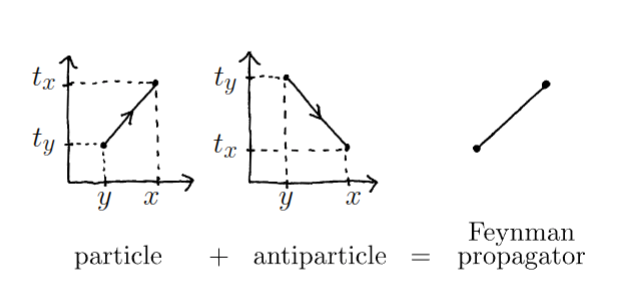
\includegraphics[width = 0.5\textwidth]{figure/费曼传播子.png}
\end{figure}

\section{\protect\hyperlink{:}{传播子与微扰论的联系}}
\addtocontents{toc}{\protect\hypertarget{:}{}}

现在让我们总结一下传播子与微扰论之间的深刻联系。在量子场论中，传播子是微扰展开的基本组成部分，而费曼图则提供了计算这些展开项的直观方法。

考虑一个包含相互作用的量子场论，其拉格朗日量可以写为
\begin{equation*}
    \mathcal{L} = \mathcal{L}_0 + \mathcal{L}_{int}
\end{equation*}

其中 $\mathcal{L}_0$ 是自由场的拉格朗日量，$\mathcal{L}_{int}$ 是相互作用项。根据路径积分量子化，两点关联函数（即传播子）可以表示为
\begin{equation*}
    G(x,y) = \frac{\int \mathcal{D}\phi \, \phi(x)\phi(y) e^{iS[\phi]}}{\int \mathcal{D}\phi \, e^{iS[\phi]}}
\end{equation*}

其中 $S[\phi] = \int d^4x \, \mathcal{L}$ 是作用量。将相互作用项展开，我们得到
\begin{align*}
    G(x,y) &= \frac{\int \mathcal{D}\phi \, \phi(x)\phi(y) e^{iS_0} \left(1 + iS_{int} + \frac{(iS_{int})^2}{2!} + \cdots\right)}{\int \mathcal{D}\phi \, e^{iS_0} \left(1 + iS_{int} + \frac{(iS_{int})^2}{2!} + \cdots\right)} \\
    &= \frac{\langle \phi(x)\phi(y) \rangle_0 + \langle \phi(x)\phi(y) iS_{int} \rangle_0 + \cdots}{1 + \langle iS_{int} \rangle_0 + \cdots}
\end{align*}

其中 $\langle \cdots \rangle_0$ 表示在自由理论中的期望值。这个展开式的每一项都可以用费曼图来表示，而费曼传播子 $\Delta(x,y)$ 正是自由理论中的两点函数。

具体来说，在动量空间中，自由标量场的传播子为
\begin{equation*}
    \Delta(p) = \frac{i}{p^2 - m^2 + i\epsilon}
\end{equation*}

在费曼图中，这对应于一条内线。当计算散射振幅时，我们需要将所有可能的费曼图相加，每个图都由传播子和顶点因子组成。例如，在 $\phi^4$ 理论中，两点函数的微扰展开为
\begin{align*}
    G(p) &= \Delta(p) + \Delta(p) \left[ -i\lambda \int \frac{d^4k}{(2\pi)^4} \Delta(k) \right] \Delta(p) + \cdots \\
    &= \Delta(p) + \Delta(p) \Sigma(p) \Delta(p) + \Delta(p) \Sigma(p) \Delta(p) \Sigma(p) \Delta(p) + \cdots \\
    &= \frac{\Delta(p)}{1 - \Sigma(p)\Delta(p)} = \frac{i}{p^2 - m^2 - \Sigma(p) + i\epsilon}
\end{align*}

其中 $\Sigma(p)$ 是自能函数，包含了所有不可约图的贡献。这个结果展示了传播子如何通过微扰修正得到重整化。

传播子与微扰论的这种联系是量子场论的核心思想之一。它不仅提供了计算物理可观测量的具体方法，还揭示了量子场论中粒子概念的深层含义：粒子是自由理论中的激发，而相互作用则通过传播子的修正来体现。这种图像在重整化群理论中得到了进一步发展，成为理解量子场论大尺度行为的关键。
